\section{Data Handling for the Receiver}
\label{DataHandlingReceiver}

Figure \ref{fig:DHR}, on page \pageref{fig:DHR}, shows the data handling structure for any receiver satellite during nominal operating conditions. Nominal operating conditions refer to the state without any system failures. The rest of this section will contain some comments of the diagram is Figure \ref{fig:DHR}.

This diagram is very similar to the diagram for the emitter found on page \pageref{fig:DHE}. The main difference is the removal of the laser payload and of several storage units. The other main difference is the lack of an X-band array, instead only the S-band antennae remain. The command arrow going from the S-band antennae to the computer consists entirely of the commands send from the emitter, whereas the command arrow going toward the S-band antennae only contains commands meant for the antennae software. Also housekeeping data arrow from the S-band to the computer is data concerning only the antennae.

\begin{figure}
\centering
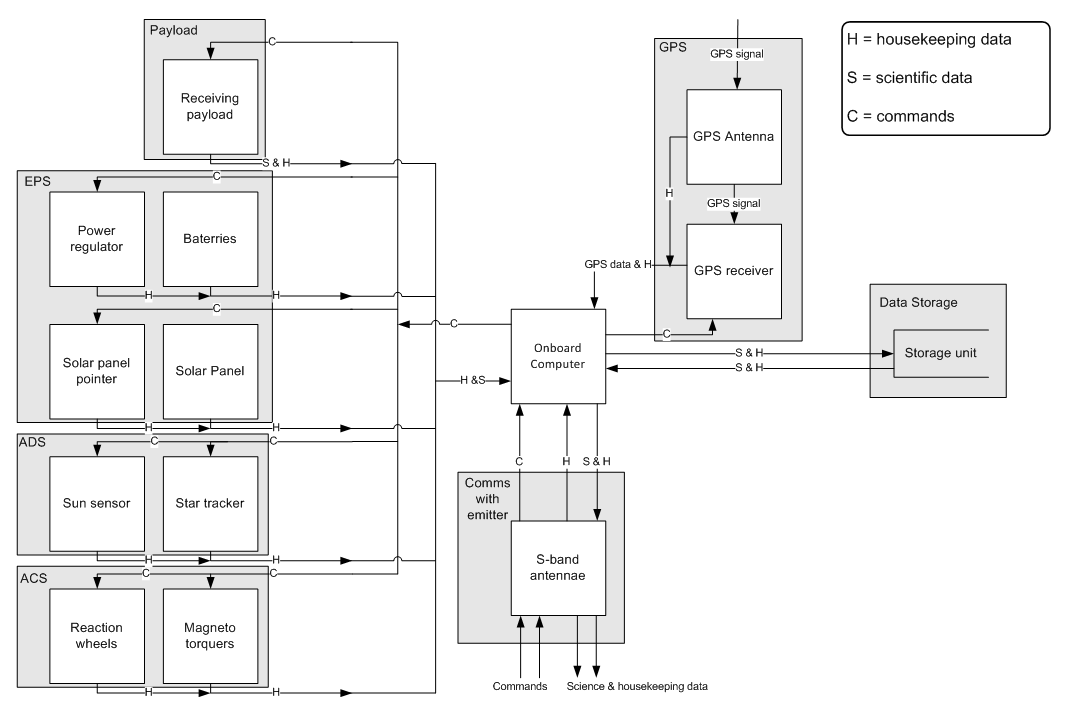
\includegraphics[width=1.0\textwidth, angle=90]{img/DHReceiver.png}
\caption{Figure showing the data handling structure for a receiver.}
\label{fig:DHR}
\end{figure}